\documentclass[11pt, dvipsnames, handout]{beamer}
\newtoggle{full}
\settoggle{full}{true}

\newtoggle{covered}
\settoggle{covered}{false}

\newtoggle{presentable}
\settoggle{presentable}{false}

\newtoggle{dualscreen}
\settoggle{dualscreen}{false}

\usepackage{pgfplots}
%\pgfplotsset{compat = newest}

\usepackage{pgfpages}

\setbeamertemplate{note page}{\pagecolor{yellow!5}\vfill \insertnote \vfill}
\usepackage{collect}
\definecollection{notes}
\newcounter{notestaken}

\usepackage{xpatch}

\usepackage{ulem}

\usepackage[framemethod=tikz]{mdframed}

\usepackage{scalerel}
\usepackage{calc}

%\usepackage{enumitem}
\setlength\fboxsep{.2em}

\usepackage{graphicx} % Allows including images
\usepackage{booktabs} % Allows the use of \toprule, \midrule and \bottomrule in tables

\xpatchcmd{\itemize}
  {\def\makelabel}
  {\setlength{\itemsep}{0.65 em}\def\makelabel}
  {}
  {}


\xpatchcmd{\beamer@enum@}
  {\def\makelabel}
  {\setlength{\itemsep}{0.65 em}\def\makelabel}
  {}
  {}


%\makeatletter
%\renewcommand{\itemize}[1][]{%
%  \beamer@ifempty{#1}{}{\def\beamer@defaultospec{#1}}%
%  \ifnum \@itemdepth >2\relax\@toodeep\else
%    \advance\@itemdepth\@ne
%    \beamer@computepref\@itemdepth% sets \beameritemnestingprefix
%    \usebeamerfont{itemize/enumerate \beameritemnestingprefix body}%
%    \usebeamercolor[fg]{itemize/enumerate \beameritemnestingprefix body}%
%    \usebeamertemplate{itemize/enumerate \beameritemnestingprefix body begin}%
%    \list
%      {\usebeamertemplate{itemize \beameritemnestingprefix item}}
%      {%
%        \setlength\topsep{1em}%NEW
%        \setlength\partopsep{1em}%NEW
%        \setlength\itemsep{1em}%NEW
%        \def\makelabel##1{%
%          {%
%            \hss\llap{{%
%                \usebeamerfont*{itemize \beameritemnestingprefix item}%
%                \usebeamercolor[fg]{itemize \beameritemnestingprefix item}##1}}%
%          }%
%        }%
%      }
%  \fi%
%  \beamer@cramped%
%  \raggedright%
%  \beamer@firstlineitemizeunskip%
%}
%
%
%
%
%
%\makeatother

%\setlist[beamer@enum@]{topsep=1 em}
%\let\origcheckmark\checkmark %screw you dingbat
%\let\checkmark\undefined %screw you dingbat
%\usepackage{dingbat} 
%\let\checkmark\origcheckmark %screw you dingbat






%\usepackage{fontawesome}

\usepackage{mathtools}
\usepackage{etoolbox, calculator}

\usepackage{xcolor}
\usepackage{tikz}
\usetikzlibrary{arrows.meta}
\usetikzlibrary{calc}
\usepackage[nomessages]{fp}
\usepackage{transparent}
\usepackage{accsupp}
%\usepackage{color, xcolor}

%colorblind-friendly palette
%\definecolor{dblue}{RGB}{51,34,136}
\definecolor{lblue}{RGB}{136,204,238}
%\definecolor{green}{RGB}{17,119,51}
\definecolor{tan}{RGB}{221,204,119}
%\definecolor{mauve}{RGB}{204,102,119}

\usepackage{tcolorbox}



\usepackage{xifthen}
\usepackage{nicefrac}
\usepackage{amsmath}
\usepackage{amsthm}
\usepackage{amssymb}
\theoremstyle{definition}
\newtheorem*{define}{Definition}
\newtheorem*{recall}{Recall}


\DeclareMathOperator{\tr}{tr}

\usepackage{multicol}
%\setlength{\columnsep}{1cm}

\usepackage{tablists, amsmath,vwcol, cancel, polynom}
\usetikzlibrary{shapes, patterns, decorations.shapes}
%\usepackage{tikzpeople}
\tikzstyle{vertex}=[shape=circle, minimum size=2mm, inner sep=0, fill]
\tikzstyle{opendot}=[shape=circle, minimum size=2mm, inner sep=0, fill=white, draw]

% common math quick commands
\newcommand{\nicedd}[2]{\nicefrac{\text{d}#1}{\text{d}#2}}
\newcommand{\dd}[2]{\dfrac{\text{d}#1}{\text{d}#2}}
\newcommand{\pd}[2]{\dfrac{\partial #1}{\partial#2}}
\renewcommand{\d}[1]{\text{d}#1}
\newcommand{\ddn}[3]{\dfrac{\text{d}^{#3}#1}{\text{d}#2^{#3}}}
\newcommand{\pdn}[3]{\dfrac{\partial^{#3}#1}{\partial#2^{#3}}}
\newcommand{\p}[0]{^{\prime}}
\newcommand{\pp}[0]{^{\prime\prime}}
\newcommand{\op}[2][\text{L}]{#1 \left[ #2 \right]}

\newcommand{\lap}[1]{\mathcal{L}\left\{#1\right\}}
\newcommand{\lapinv}[1]{\mathcal{L}^{-1}\left\{#1\right\}}
\newcommand{\lapint}[1]{\int_0^\infty e^{-st}#1dt}
\newcommand{\evalat}[2]{\Big|_{#1}^{#2}}

\newcommand{\paren}[1]{ \left( #1 \right)}

\newcommand{\haxis}[4][\normcolor]{\draw[#1, <->] (-#2,0)--(#3,0) node[right]{$#4$}; }

\newcommand{\circled}[1]{\raisebox{.5pt}{\textcircled{\raisebox{-.9pt} {#1}}}}
\newcommand{\axis}[4]{\draw[\normcolor, <->] (-#1,0)--(#2,0) 
node[right]{$x$};
\draw[help lines, <->] (0,-#3)--(0,#4) node[above]{$y$};}

\newcommand{\laxis}[6]{\draw[<->] (-#1,0)--(#2,0) 
node[right]{$#5$};
\draw[ <->] (0,-#3)--(0,#4) node[above]{$#6$};}
\newcommand{\xcoord}[2]{
	\draw (#1,.2)--(#1,-.2) node[below]{$#2$};}
\newcommand{\textnode}[3]{
	\draw (#1,#2) node[below]{$#3$};}
	
\newcommand{\nxcoord}[2]{
	\draw (#1,-.2)--(#1,.2) node[above]{$#2$};}
\newcommand{\ycoord}[2]{
	\draw (.2,#1)--(-.2,#1) node[left]{$#2$};}
\newcommand{\nycoord}[2]{
	\draw (-.2,#1)--(.2,#1) node[right]{$#2$};}
\newcommand{\dlim}{\displaystyle\lim}
\newcommand{\dlimx}[1]{\displaystyle\lim_{x \rightarrow #1}}
\newcommand{\stickfig}[2]{
	\draw (#1,#2) arc(-90:270:2mm);
	\draw (#1,#2)--(#1,#2-.5) (#1-.25,#2-.75)--(#1,#2-.5)--(#1+.25,#2-.75) (#1-.2,#2-.2)--(#1+.2,#2-.2);}	

%\newcounter{example}
%\setcounter{example}{1}
%\newcounter{preFrameExample}
%\AtBeginEnvironment{frame}{\setcounter{preFrameExample}{\value{example}}}
%\newcommand{\ex}[1]{
%	 \setcounter{example}{\value{preFrameExample}}
%	 \textcolor{green}{\small\fbox{Example \arabic{example}: #1}}\\[8pt]
%	\stepcounter{example}}
%\newcommand{\exans}[1]{
%	\SUBTRACT{\value{preFrameExample}}{1}{\n}
%	 \textcolor{green}{\small\fbox{Solution \n: #1}}\\[8pt]}
\mode<presentation> {

% The Beamer class comes with a number of default slide themes
% which change the colors and layouts of slides. Below this is a list
% of all the themes, uncomment each in turn to see what they look like.


\usetheme{CambridgeUS}
\usecolortheme[named=black]{structure}


\newcommand{\studentcolor}[0]{ForestGreen}
\newcommand{\normcolor}[0]{NavyBlue}
\newcommand{\alertcolor}{Red}

\setbeamercolor{normal text}{fg=\normcolor}
\setbeamercolor{frametitle}{fg=\normcolor}
\setbeamercolor{section in head/foot}{fg=Black, bg=Gray!20}
\setbeamercolor{subsection in head/foot}{fg=Green!70!Black, bg=Gray!10}
\setbeamercolor{alerted text}{fg=\alertcolor}
\setbeamerfont{alerted text}{series=\bf}
\setbeamertemplate{enumerate items}[default]
\setbeamercolor{enumerate item}{fg=\normcolor}

\setbeamertemplate{footline} % To remove the footer line in all slides uncomment this line
%\setbeamertemplate{footline}[page number] % To replace the footer line in all slides with a simple slide count uncomment this line

\setbeamertemplate{navigation symbols}{} % To remove the navigation symbols from the bottom of all slides uncomment this line
}

\newcommand{\alertbox}[1]{\tcbox[on line, colframe=\alertcolor, colback=White, left=2pt,right=2pt,top=2pt,bottom=2pt]{\usebeamercolor*{normal text}#1}}


\newcommand{\startstu}{\setbeamercolor{normal text}{fg=\studentcolor}\usebeamercolor*{normal text}\setbeamercolor{enumerate item}{fg=\studentcolor}\usebeamercolor*{enumerate item}}
\newcommand{\stopstu}{\setbeamercolor{normal text}{fg=\normcolor}\usebeamercolor*{normal text}\setbeamercolor{enumerate item}{fg=\normcolor}\usebeamercolor*{enumerate item}}

\newcommand{\takenote}[1]{ \begin{collect}{notes}{}{}{}{}  #1  \end{collect}  \addtocounter{notestaken}{1}} %\ifthenelse{\value{notestaken}>0}{\hrulefill\\}{}

\makeatletter
\newcommand{\cover}{\alt{\beamer@makecovered}{\beamer@fakeinvisible}}
\newcommand{\ucover}[1]{\iftoggle{full}{}{\beamer@endcovered} \stopstu #1\startstu \iftoggle{full}{}{\beamer@startcovered} }
%\newcommand{\ucover}[1]{\beamer@endcovered \stopstu #1\startstu \beamer@startcovered }
\makeatother

\newcommand{\skippause}{ \addtocounter{beamerpauses}{-1}}
\newcommand{\blockpres}{ \skippause \pause }

\newcommand{\studentify}[1]{\startstu #1  \stopstu }
\newcommand{\student}[1]{\iftoggle{full}{ \pause  \studentify{#1} }{\iftoggle{covered}{\studentify{#1}}{\cover{  #1 }}}}
\newcommand{\cstudent}[1]{\student{\begin{center} #1 \end{center}}}
\newcommand{\fullonly}[1]{\iftoggle{full}{ #1}{}}
\newcommand{\presentonly}[1]{\iftoggle{presentable}{ #1}{}}

\usepackage{xparse}
\usepackage{xifthen}

% shortcuts for commonly-used presentation elements
%\NewDocumentCommand{\slide}{o m}
% {\IfValueTF{#1}{\begin{frame}[t]{#1}}{\begin{frame}[t]} #2 \end{frame}}

\newtoggle{iscovered}

\newcommand{\slide}[2][]{%
%\setcounter{notestaken}{0}
\takenote{#2} 
%\ifthenelse{\equal{#1}{}}{\begin{frame}[t]}{\begin{frame}[t]{#1}} #2 \ifthenelse{\value{notestaken}>0}{ \note{\includecollection{notes}}}{} \end{frame}%
\ifthenelse{\equal{#1}{}}{\begin{frame}[t]}{\begin{frame}[t]{#1}} #2 \iftoggle{covered}{\settoggle{iscovered}{true}}{\settoggle{iscovered}{false}}  \note{ \iftoggle{iscovered}{}{\settoggle{covered}{true}} #2 \iftoggle{iscovered}{}{\settoggle{covered}{false}} } \end{frame}%
%\setcounter{notestaken}{0}
}
\newcommand{\defn}[2][]{%
 \setcounter{listcounter}{0}%
\ifthenelse{\equal{#1}{}}{\begin{block}{Definition}}{\begin{block}{#1 :}}%
 #2 \vspace{0.25em} \ifthenelse{\value{listcounter}>0}{\skippause}{} \pause \end{block}%
}



\newcommand{\arr}[2]{\begin{array}{#1}#2\end{array}}
\newcommand{\mat}[2]{\left[\arr{#1}{#2}\right]}
\newcommand{\carray}[1]{\arr{c}{#1}}
\newcommand{\larray}[1]{\arr{l}{#1}}
\newcommand{\rarray}[1]{\arr{r}{#1}}
\newcommand{\colvec}[1]{\mat{c}{#1}}

\newcommand{\itmz}[1]{\addtocounter{listcounter}{1} \begin{itemize}#1 \end{itemize} }
\newcommand{\subitem}[1]{\addtocounter{listcounter}{1} \begin{itemize} \item #1 \end{itemize}}
%
\newcommand{\enum}[1]{\addtocounter{listcounter}{1} \begin{enumerate} #1  \end{enumerate}  }


\newcommand{\algnlbl}[1]{\begin{align}#1  \end{align}} 
\newcommand{\algn}[1]{\begin{align*}#1  \end{align*}} 
\newcommand{\lgn}[1]{ \action<+->{#1} }
\newcommand{\slgn}[1]{\iftoggle{full}{\action<+->{ \startstu #1 \stopstu}}{ \cover{ #1 } } \takenote{$#1$}}

\newcommand{\chckmrk}{\alert{\checkmark}}

\usepackage{pifont}
\newcommand{\xmark}{\alert{\text{\large \ding{55}}}}

\newcommand{\return}[0]{\raisebox{.5ex}{\rotatebox[origin=c]{180}{$\Lsh$}}}
\usepackage{pbox}
%\newcommand{\ex}[1]{\rotatebox[origin=c]{10}{\uline{ex}}:$\;$\pbox[t][][b]{0.9\linewidth}{#1}}
\newcommand{\ex}[1]{\uline{ex}:$\;$\pbox[t][][t]{0.9\linewidth}{#1}}
\newcommand{\eg}[1]{e.g.,$\;$\pbox[t][][t]{0.9\linewidth}{#1}}
\newcommand{\tikzplot}[8][]{%
\begin{tikzpicture}

\begin{scope}[]%
\clip(-#2,-#4) rectangle (#3,#5);%
#8%
\end{scope}%
\laxis{#2}{#3}{#4}{#5}{#6}{#7}%
#1
\end{tikzpicture}%
}


\newcommand{\cancelslide}[1]{%
\begingroup%
\setbeamertemplate{background canvas}{%
\begin{tikzpicture}[remember picture,overlay]%
\draw[line width=2pt,red!60!black] %
  (current page.north west) -- (current page.south east);%
\draw[line width=2pt,red!60!black] %
  (current page.south west) -- (current page.north east);%
\end{tikzpicture}}%
#1%
\endgroup%
}
\renewcommand{\CancelColor}{\color{red}}
\newcommand{\twocols}[3][0.5]{\begin{columns}\begin{column}{#1\textwidth}#2\end{column}\hspace{1em}\vrule{}\hspace{1em}\begin{column}{#1\textwidth}#3\end{column}\end{columns}}

\newcommand{\twomini}[5][1]{\calculatespace \begin{minipage}[t]{\columnwidth}\begin{minipage}[][#1\contentheight][t]{#2\columnwidth}#4\end{minipage}\hfill\begin{minipage}[][#1\contentheight][t]{#3\columnwidth}#5\end{minipage}\end{minipage}}

\newcommand{\threemini}[7][1]{\calculatespace \begin{minipage}[t]{\columnwidth}\begin{minipage}[][#1\contentheight][t]{#2\columnwidth}#5\end{minipage}\hfill\begin{minipage}[][#1\contentheight][t]{#4\columnwidth}#6\end{minipage}\hfill\begin{minipage}[][#1\contentheight][t]{#3\columnwidth}#7\end{minipage}\end{minipage}}


\newcounter{listcounter}
\setcounter{listcounter}{0}



\newif\ifsidebartheme
\sidebarthemetrue

\newdimen\contentheight
\newdimen\contentwidth
\newdimen\contentleft
\newdimen\contentbottom
\makeatletter
\newcommand*{\calculatespace}{%
\contentheight=\paperheight%
\ifx\beamer@frametitle\@empty%
    \setbox\@tempboxa=\box\voidb@x%
  \else%
    \setbox\@tempboxa=\vbox{%
      \vbox{}%
      {\parskip0pt\usebeamertemplate***{frametitle}}%
    }%
    \ifsidebartheme%
      \advance\contentheight by-1em%
    \fi%
  \fi%
\advance\contentheight by-\ht\@tempboxa%
\advance\contentheight by-\dp\@tempboxa%
\advance\contentheight by-\beamer@frametopskip%
\ifbeamer@plainframe%
\contentbottom=0pt%
\else%
\advance\contentheight by-\headheight%
\advance\contentheight by\headdp%
\advance\contentheight by-\footheight%
\advance\contentheight by4pt%
\contentbottom=\footheight%
\advance\contentbottom by-4pt%
\fi%
\contentwidth=\paperwidth%
\ifbeamer@plainframe%
\contentleft=0pt%
\else%
\advance\contentwidth by-\beamer@rightsidebar%
\advance\contentwidth by-\beamer@leftsidebar\relax%
\contentleft=\beamer@leftsidebar%
\fi%
}
\makeatother


\iftoggle{dualscreen}{\setbeameroption{show notes on second screen=right}}{}


\begin{document}

\section{Lecture 23}
\subsection{Introduction}
\settoggle{covered}{true}
\slide[Partial Differential Equations (PDEs)]{
A PDE is a DE for a function $u\left(x_1, x_2,\dots \right)$ that depends on 2 or more independent variables and contains partial derivatives taken with respect to at least 2 variables.\vfill
\student{
\ex{1D Heat Equation}\[\pd{}{t}u(x,t) = \alpha \pdn{}{x}{2}u(x,t)\]or
\[u_t = \alpha u_{xx}\]

\vfill
Partial derivatives are used so we get the same results in non-euclidean coordinates (e.g., speherical, polar, etc) \vfill

\vfill
Trick: convert PDE into an (infinite) system of ODEs and solve those ODEs instead.

}
}
\settoggle{covered}{false}
\slide[1D Heat Equation - An Initial Boundary Value Problem]{
Let $u(x,t)$ be the temperature at the position $x\in\student{\underbrace{\ucover{[0,L]}}_{\text{domain}}}$ and the time t\vfill
The heat equation tells us the evolution of the  temperature distribution throughout the domain (e.g., a 1D rod) from some initial condition $u_0(x)$.
\algn{ &\qquad\quad \student{\text{(Homogeneous)}}\\& \qquad \text{\uline{Boundary Conditions}}\quad && \text{\uline{Initial Condition}}\\
\larray{u_t= \alpha u_{xx}\\\text{for } x\in(0,L)} \; \text{with }& \larray{\student{\overbrace{\ucover{u(0,t)=u(L,t)=0}}^{\text{\large rod connected to ice baths}}} \\ \qquad \qquad \qquad  \text{\uline{or}} \\ \student{\underbrace{\ucover{u_x(0,t)=u_x(L,t)=0}}_{\quad \qquad \text{\Large insulated rod}\qquad }}} &\text{and}\quad  &u(x,0)=u_0(x)}
\vfill
\student{$\alpha=$ thermal diffusivity}
}
\subsection{Separation of Variables}


\slide[Separation of Variables]{\vspace{-1.5em}
\[\pd{}{t}u(x,t) = \alpha \pdn{}{x}{2}u(x,t) \]
 \vfill
Guess: $u(x,t) = X(x)T(t)$\algn{
X(x)T\p(t)&=\alpha X\pp(x)T(t)\\\\
\frac{T\p(t)}{\alpha T(t)} &= \frac{X\pp(x)}{X(x)}}\vfill
\student{
This can only be true  if each fraction is a constant\vfill
\[ \frac{T\p(t)}{ \alpha T(t)} =  \frac{X\pp(x)}{X(x)} = -\lambda \qquad \Leftrightarrow \qquad \rarray{  X\pp(x) + \lambda X(x)=0\\ \text{and} \qquad \qquad \text{~} \\T'(t) =-  \alpha \lambda T(t)  }\]
}
}


\slide[$X\pp + \lambda X = 0\quad $ \small with BCs:  \hfill $X(0)=X(L)=0$ \hfill or \hfill $X\p(0)=X\p(L)=0$]{\vspace{-1em}

Non-zero solutions exist only for $\lambda=\lambda_n = \left(\frac{n\pi}{L}\right)^2$ with $n\in\mathbb{N^+}$ or $n=0$.\vfill
$\uline{\lambda = 0}$
\[ X_0\pp = 0 \]\vspace{-1em}
\student{\[X_0(x) = A_0 + \cancelto{\text{does not match BCs}}{B_0x}\]\vfill}
$\uline{\lambda > 0}$
\[X_n\pp  + \lambda_n X_n  = 0 \qquad \text{try}\qquad X_n (x) =c_n e^{rx}\]\vfill
\twomini[.55]{.5}{.4}{
\student{
\algn{ r^2 + \lambda_n &=0 \qquad \Rightarrow r=\pm i\sqrt{\lambda_n}\\ \\ X_n(x) &= A_n \cos \left(\frac{n \pi}{L}x\right) + B_n \sin\left( \frac{ n\pi}{L} x\right)  }
\vfill \centering Choose $\sin$ or $\cos$ based on the BCs of the problem.\vfill
}

}{

\tikzplot[\xcoord{3.14159}{L}]{.1}{3.5}{.75}{.75}{x}{\sin(n\pi x/L)}{
\draw[domain=0:3.14159, red, samples=200, smooth, thick] plot ({\x,0.5*sin(deg(\x))}) node[xshift=-3.75em, yshift=1.6em, fill=white, inner sep=0.3]{ \tiny $n=1$};
\draw[domain=0:3.14159, red, samples=200, smooth, thick, dashed] plot ({\x,0.5*sin(deg(2*\x))}) node[xshift=-4.5em, yshift=.5em, fill=white, inner sep=0.3]{ \tiny $n=2$};
\draw[domain=0:3.14159, red, samples=200, smooth, thick, dotted] plot ({\x,0.5*sin(deg(3*\x))})node[xshift=-6em, yshift=-.7em, fill=white, inner sep=0.3]{ \tiny $n=3$};
}

\tikzplot[\xcoord{3.14159}{\;\;L}]{.1}{3.5}{.75}{.75}{x}{\cos(n\pi x/L)}{
\draw[domain=0:3.14159, blue, samples=200, smooth, thick] plot ({\x,0.5*cos(deg(\x))}) node[xshift=-6em, yshift=2.65em, fill=white, inner sep=0.3]{ \tiny $n=1$};
\draw[domain=0:3.14159, blue, samples=200, smooth, thick, dashed] plot ({\x,0.5*cos(deg(2*\x))}) node[xshift=-6.15em, yshift=-.95em, fill=white, inner sep=0.3]{ \tiny $n=2$};
\draw[domain=0:3.14159, blue, samples=200, smooth, thick, dotted] plot ({\x,0.5*cos(deg(3*\x))}) node[xshift=-7.2em, yshift=.5em, fill=white, inner sep=0.3]{ \tiny $n=3$};
}

}\vfill 


}


\slide[ Time-Dependence + Superposition]{\vspace{-2.5em}
\[u_n(x,t)=T_n(t)X_n(x) \quad \text{ with } \quad T_n\p = - \alpha \lambda_n T  \quad \Leftrightarrow  \quad T_n(t)=c_ne^{-\alpha \lambda_n t}\]
\student{\[u_n(x,t)=c_ne^{-\alpha \omega_n^2 t} \left(A_n \cos \left( \omega_n x\right) +  B_n \sin\left(  \omega_n  x\right) \right)\]}\vfill
We have infinitely many solutions to the linear PDE, any linear combinations of those solutions is also a solution
\student{\[u(x,t) = \sum_{n=1}^\infty u_n(x,t) \]}
\vfill
Initial condtion: $u(x,0)=u_0(x)$
\student{Pick $c_n=1 \quad$(without loss of generality)
\[u_0(x) = A_0 + \sum_{n=1}^\infty \left( A_n \cos \left( \omega_i x\right)   +  B_n \sin\left(  \omega_n  x\right) \right) \qquad \omega_n=\frac{ n\pi}{L} \]

Find $A_n$ and $B_n$  by taking a Fourier Series expansion of $u_0(x)$

}
}


\subsection{Periodic Extensions}
\slide[ICs + BCs $\Rightarrow$ Periodic extension]{\vspace{-2em}
\[u_0(x) = A_0 + \sum_{i=n}^\infty \left( A_n \cos \left( \omega_inx\right)   +  B_n \sin\left(  \omega_n  x\right) \right) \qquad \omega_n=\frac{ n\pi}{L} \]
$u_0(x)$ is defined for $x\in[0,L]$ only.\vfill
\student{Our spatial solution is the Fourier Series of a 2L periodic function!}
\vfill BCs:  \hfill $X(0)=X(L)=0$ \hfill or \hfill $X\p(0)=X\p(L)=0$
\twomini[.6]{.6}{.4}{
\student{\vfill\itmz{ \item $\sin$ terms satisfy $X(0)=X(L)=0$ \enum{\item Extend $u_0(x)$ as an \uline{odd} function \item Take its FS:  \uline{Fourier Sine Series}}\vfill
\item $\cos$ terms satisfy $X\p(0)=X\p(L)=0$ \enum{\item Extend $u_0(x)$ as an \uline{even} function \item Take its FS:  \uline{Fourier Cosine Series}} }\vfill
 }}{\centering 
\tikzplot[\xcoord{1.2}{L} \xcoord{-1.2}{-L}]{1.75}{1.75}{1.2}{1.2}{x}{}{
\draw[domain=0:1.2,  samples=2, smooth, thick] plot ({\x,\x)}) node[xshift=-.35em, yshift=-2em, fill=white, inner sep=0.3]{ \tiny $u_0(x)=x$};
\student{\draw[domain=-1.2:0,  samples=2, smooth, thick] plot ({\x,\x)}) node[xshift=1.2em, yshift=-2em, fill=white, inner sep=0.3]{ \tiny odd periodic extension};}
}
\tikzplot[\xcoord{1.2}{L} \xcoord{-1.2}{-L}]{1.75}{1.75}{.1}{1.2}{x}{}{
\draw[domain=0:1.2,  samples=2, smooth, thick] plot ({\x,\x)}) node[xshift=-.35em, yshift=-2em, fill=white, inner sep=0.3]{ \tiny $u_0(x)=x$};
\student{\draw[domain=-1.2:0,  samples=2, smooth, thick] plot ({\x,-\x)}) node[xshift=-.2em, yshift=2em, fill=white, inner sep=0.3]{ \tiny even periodic extension};}
}
}
}

\subsection{Solution to the heat equation with homogeneous BCs}
\slide[ Solution to \hfill $u_t=\alpha u_{xx}$ \hfill $\larray{ \text{with } 0<x<L  \\ \text{and }u(x,0)=u_0(x)}$ \hfill]{\vspace{-1em}
\[u(x,t)=\frac{a_0}{2} + \sum_{n=1}^\infty e^{-\alpha \frac{n^2\pi^2}{L^2} t} \left( a_n \cos\left(\frac{n\pi}{L} x\right) +  b_n \sin\left(\frac{n\pi}{L} x\right) \right)  \]\vfill
If $u(0,t)=u(L,t)=0$: $\quad$ Fourier sine series \hfill ~
\algn{a_n &= 0\\b_n&=\frac{2}{L}\int_0^L u_0(x) \sin\paren{\frac{n\pi}{L}x} dx }\vfill
If $u_x(0,t)=u_x(L,t)=0$: $\quad$ Fourier cosine series \hfill ~
\algn{a_n &= \frac{2}{L}\int_0^L u_0(x) \cos\paren{\frac{n\pi}{L}x} dx\\b_n&=0 }

}

\slide[ ]{\vspace{-.5em}
\ex{$u_t=\alpha u_{xx}\quad $  for $ 0<x<L \qquad $ with  $u(x,0)=x$ }

\vspace{.6em}
Two possible homogeneous BCs:

\vspace{.6em}
\twomini[.7]{.5}{.5}{ $u(0,t)=u(L,t)=0$
\student{
\algn{u(x,t) &=\\& \sum_{n=1}^\infty e^{-\alpha \frac{n^2\pi^2}{L^2} t}  b_n \sin\left(\frac{n\pi}{L} x\right)  \\\\
b_n &= \frac{2}{L} \int_0^L x \sin\paren{\frac{n\pi x}{L}} dx \\
& = -L \frac{2  (-1)^n}{\pi  n}}
}

}{$u_x(0,t)=u_x(L,t)=0$
\vspace{-.5em}
\student{
\algn{u(x,t) &=\frac{a_0}{2}\\& \phantom{=} +\sum_{n=1}^\infty e^{-\alpha \frac{n^2\pi^2}{L^2} t}  a_n \cos\left(\frac{n\pi}{L} x\right)  \\\\
a_n &= \frac{2}{L} \int_0^L x \cos\paren{\frac{n\pi x}{L}} dx \\
& =\frac{2 L \left((-1)^n-1\right)}{\pi ^2 n^2}\\\\
a_0&=\frac{2}{L} \int_0^L x  dx = L }
}

}

}
\settoggle{covered}{false}
\slide[ ]{\vspace{-.5em}
\ex{$u_t=\alpha u_{xx}\quad $  for $ 0<x<L \qquad $ with  $\larray{u(x,0)=\sin(5\pi x/L)\\ u(0,t)=u(L,t)=0}$ }

\student{
From the BCs,
\[u(x,t)= \sum_{n=1}^\infty e^{-\alpha \frac{n^2\pi^2}{L^2} t}  b_n \sin\left(\frac{n\pi}{L} x\right) \]

\algn{b_n&=\frac{2}{L}\int_0^L\sin(5\pi x/L) \sin(\frac{n\pi}{L}x) dx\\
&=\begin{cases} 1 & \text{if } n=5\\
0&\text{otherwise}\end{cases} \\\\
u(x,t) &= e^{-\alpha \frac{25\pi^2}{L^2} t}   \sin\left(\frac{5\pi}{L} x\right)}
}

}

%
%\slide{
%We  previously saw some 2L-periodic extensions of $f(x)=x$ for $x\in[0,L]$
%\vfill
%
%\twomini[.72]{.48}{.48}{
%
%Even extension - \small reflect about $y$-axis
%\vfill
%
%\centerline{\tikzplot[\xcoord{-1}{-L} \xcoord{1}{L}]{2.65}{2.65}{1.05}{1.05}{x}{f(x)=f(-x)}{
%
%
%
%\foreach \i in {-2,-1,0,1,2}{
%
%\draw[domain=0:1,  thick, lblue] plot ({\x-2*\i},{\x});
%\draw[domain=-1:0, thick, lblue] plot ({\x-2*\i},{-\x});
%
%
%}
%\draw[ ultra thick] (0,0)--(1,1);
%}
%}
%
%\vfill
%\centerline{\tikzplot{2.65}{2.656}{1.05}{1.05}{x}{f(x)\approx  \frac{L}{2} + \frac{2L}{\pi^2} \overset{3}{\underset{n=1 }{\sum} } \frac{(-1)^n-1}{n^2}\cos\left( \frac{n\pi}{L}x\right)}{
%
%
%
%\foreach \i in {-2,-1,0,1,2}{
%
%\draw[domain=0:1] plot ({\x-2*\i},{\x});
%\draw[domain=-1:0] plot ({\x-2*\i},{-\x});
%
%
%}
%
%\draw[domain=-3:3, red, samples=200, smooth, thick] plot ({\x},{ 1/2  - 4/(3.141459^2)*cos((3.141459)*deg(\x))    -  4/(9*3.141459^2)*cos(3*(3.141459)*deg(\x))     });
%
%
%}
%}
%}{
% Odd extension - \small reflect about both axes
%\vfill
%\centerline{\tikzplot[\xcoord{-1}{-L} \xcoord{1}{L}]{2.65}{2.65}{1.05}{1.05}{x}{f(x)=-f(-x)}{
%
%
%
%\foreach \i in {-2,-1,0,1,2}{
%
%\draw[domain=-1:1, thick, YellowOrange] plot ({\x-2*\i},{\x});
%\draw[dashed, thick, YellowOrange] ({2*(\i-1)+1},1)--({2*(\i-1)+1},-1);
%
%}
%\draw[ ultra thick] (0,0)--(1,1);
%}
%}
%
%\vfill
%
%\centerline{\tikzplot{2.65}{2.656}{1.05}{1.05}{x}{f(x)\approx  -L  \overset{15}{\underset{n=1 }{\sum} } \frac{(-1)^n}{n\pi}\sin\left( \frac{n\pi}{L}x\right)}{
%\foreach \i in {-2,-1,0,1,2}{
%
%\draw[domain=-1:1] plot ({\x-2*\i},{\x});
%\draw[dashed,] ({2*(\i-1)+1},1)--({2*(\i-1)+1},-1);
%
%}
%
%\draw[domain=-3:3, red, samples=200, smooth, thick] plot ({\x},{(2/3.14145)*sin(3.14145*deg(\x)) - (1/3.14145)*sin(2*3.14145*deg(\x)) + (2/(3*3.14145))*sin(3*3.14145*deg(\x)) - (2/(4*3.14145))*sin(4*3.14145*deg(\x))  +  (2/(5*3.14145))*sin(5*3.14145*deg(\x))    - (2/(6*3.14145))*sin(6*3.14145*deg(\x))  +  (2/(7*3.14145))*sin(7*3.14145*deg(\x)) - (2/(8*3.14145))*sin(8*3.14145*deg(\x)) +  (2/(9*3.14145))*sin(9*3.14145*deg(\x)) -  (2/(10*3.14145))*sin(10*3.14145*deg(\x)) +  (2/(11*3.14145))*sin(11*3.14145*deg(\x))  -  (2/(12*3.14145))*sin(12*3.14145*deg(\x)) +  (2/(13*3.14145))*sin(13*3.14145*deg(\x)) -  (2/(14*3.14145))*sin(14*3.14145*deg(\x))     +  (2/(15*3.14145))*sin(15*3.14145*deg(\x))  });
%
%%\draw[domain=-6:6, red, samples=200, smooth, thick] plot ({\x},{(2/3.14145)*sin(3.14145*deg(\x)) - (1/3.14145)*sin(2*3.14145*deg(\x)) + (2/(3*3.14145))*sin(3*3.14145*deg(\x)) - (2/(4*3.14145))*sin(4*3.14145*deg(\x))  });
%
%
%}
%}
%}
%
%\vfill
%
%Any periodic function can be represented by a Fourier series.\vfill
%\centerline{High frequency terms help with discontinuities (e.g., at boundaries)}
%
%}
%
%
%\slide[]{\vspace{-.5em}
%Solve$ \qquad u_t=0.1 u_{xx} \qquad \larray{ \text{for } 0<x<L  \\ \text{and }u(x,0)=x} \qquad$ subject to BC1 and BC2 \hfill
%\vfill
%BC1: $X(0)=X(L)=0$ $\quad$\student{ Fourier sine series \hfill \tikzplot{1.65}{1.65}{.2}{.2}{x}{}{
%
%
%
%\foreach \i in {-2,-1,0,1,2}{
%
%\draw[domain=-1:1, thick] plot ({(\x-2*\i)/2},{\x/5});
%\draw[dashed, thick] ({(2*(\i-1)+1)/2},.2)--({(2*(\i-1)+1)/2},-.2);
%
%}
%
%}
%
%
%\algn{u_0(x) &= x \approx -L\sum_{n=1}^\infty  \frac{(-1)^n }{n\pi}\sin\left( \frac{n\pi}{L}x\right) \\
%u(x,t) &= -L\sum_{n=1}^\infty  e^{-0.1\frac{n^2\pi^2}{L^2} t} \frac{(-1)^n }{n\pi}\sin\left( \frac{n\pi}{L}x\right)  \qquad t>0  }}\vfill
%BC2: $X\p(0)=X\p(L)=0$ $\quad$ \student{ Fourier cosine series \hfill  \hfill \tikzplot{1.45}{1.45}{0}{.3}{x}{}{
%
%
%\foreach \i in {-2,-1,0,1,2}{
%
%\draw[domain=0:1,  thick] plot ({(\x-2*\i)/2},{\x/3.2});
%\draw[domain=-1:0, thick] plot ({(\x-2*\i)/2},{-\x/3.2});
%
%
%}
%
%}
%
%\algn{u_0(x) &= x = \frac{L}{2} + 2L\sum_{n=1}^\infty  \frac{(-1)^n -1}{n^2\pi^2}\cos\left( \frac{n\pi}{L}x\right) \\
%u(x,t) &=  \frac{L}{2} + 2L\sum_{n=1}^\infty    e^{-0.1\frac{n^2\pi^2}{L^2} t} \frac{(-1)^n -1}{n^2\pi^2}\cos\left( \frac{n\pi}{L}x\right)   \qquad t\geq0  }}\vfill
%
%}
%
%\slide[ Zero-flux Boundaries \hfill  $X\p(0)=X\p(L)=0$]{\vspace{-1.25em}
%
%\[u(x,t)=\frac{L}{2} + 2L\sum_{n=1}^\infty e^{-\alpha \omega_n^2 t}  \frac{(-1)^n-1}{n^2\pi^2}\cos\left(\omega_n x\right)  \]
%\vfill
%High-frequency terms decay the fastest \vfill $\quad \Rightarrow \quad$ Boundary conditions are imposed immediately.\vfill
%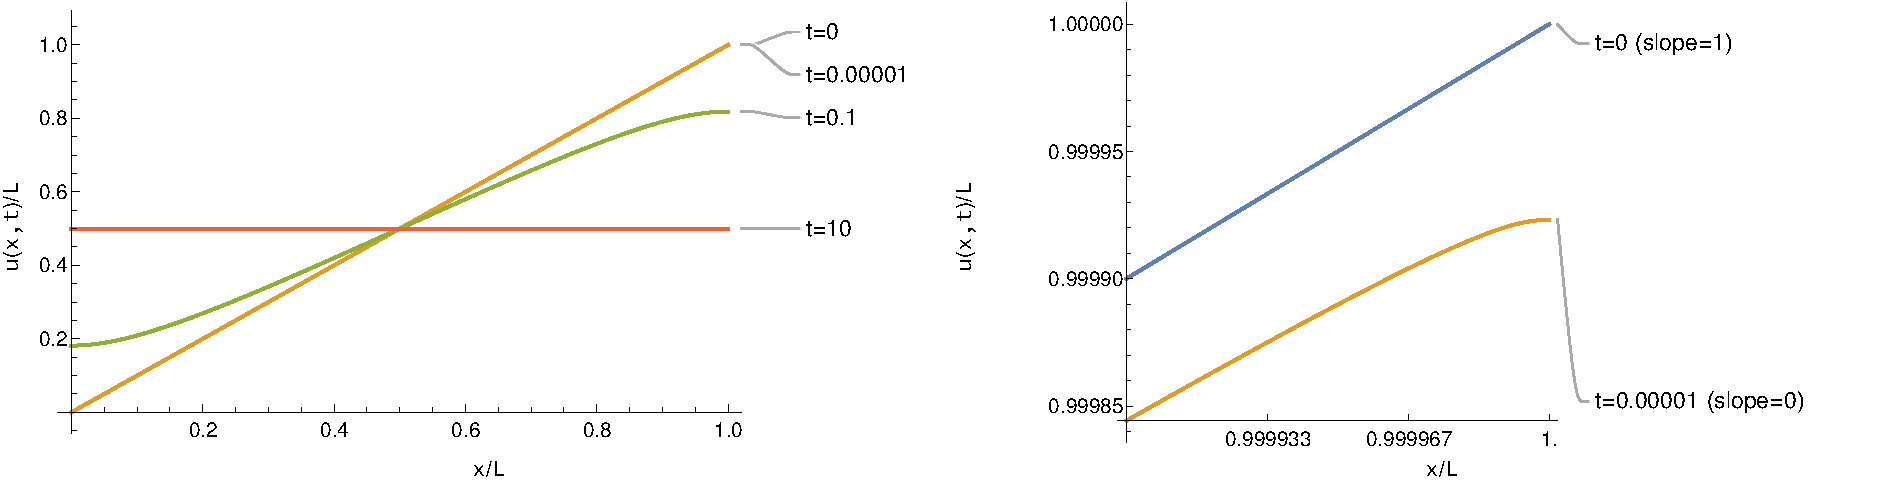
\includegraphics[width=\columnwidth]{images/zero_flux_BCs.pdf}\vfill
%Long-term Behaviour: $\qquad u(x,t)\approx \frac{L}{2} -\frac{ 4L}{\pi^2}e^{-\alpha \frac{\pi^2}{L^2} t}  \cos\left(\frac{\pi}{L} x\right)  $
%}
%
%\slide[ Clamped Boundaries \hfill  $X(0)=X(L)=0$]{\vspace{-1.25em}
%\[u(x,t)=-L\sum_{n=1}^\infty e^{-\alpha \omega_n^2 t}  \frac{(-1)^n}{n\pi}\sin\left( \omega_n x\right)  \]
%\vfill
%High-frequency terms decay the fastest \vfill $\quad \Rightarrow \quad$ Boundary conditions are imposed immediately.\vfill
%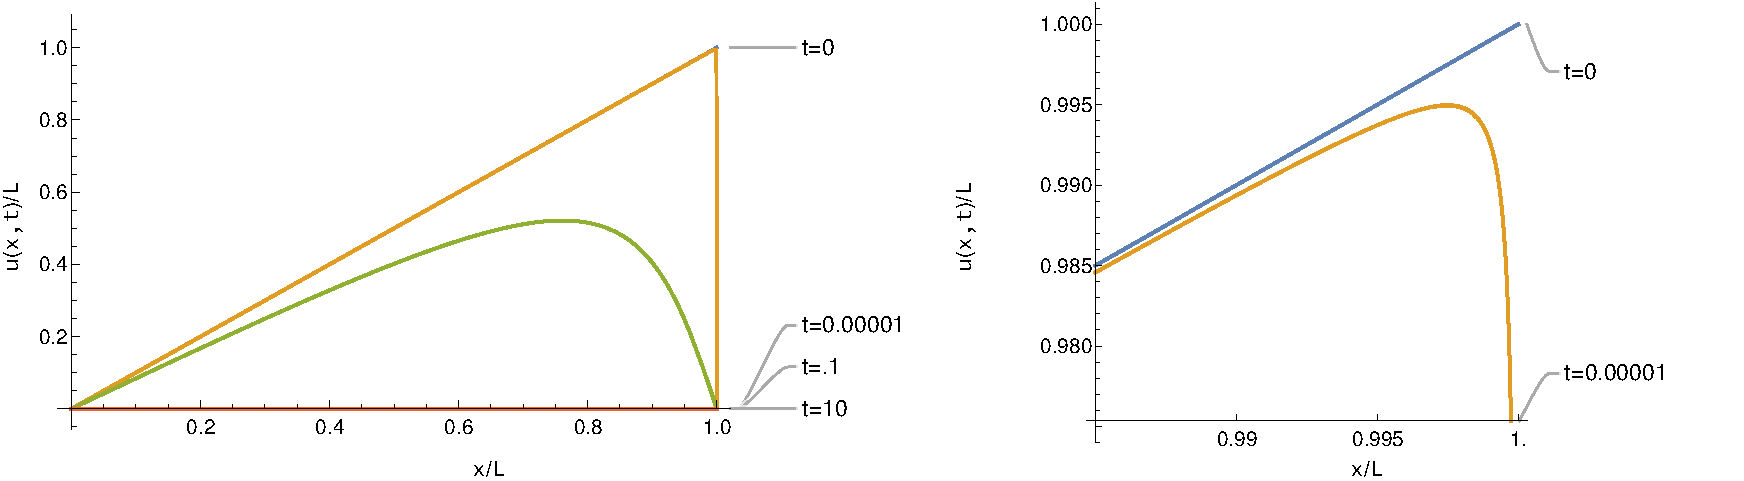
\includegraphics[width=\columnwidth]{images/clamped_BCs.pdf}\vfill
%\vfill
%Long-term Behaviour: $\qquad u(x,t)\approx \frac{ L}{\pi}e^{-\alpha \frac{\pi^2}{L^2} t}  \sin\left(\frac{\pi}{L} x\right)  $
%}
%
%
%\slide{
%\ex{\twomini[.1]{.7}{.295}{$u_t=\alpha u_{xx}$, \hspace{2em} $\arr{l}{u(0,t)=u(1,t)=0 \hspace{1em}\\u(x,0)=x(1-x) \text{ on } [0,1]}$}{\tikzplot[\xcoord{2}{\scriptscriptstyle 1}]{.1}{2.1}{.1}{1}{x\phantom{t}}{\scriptscriptstyle u(x,0)}{\draw[domain=0:1] plot (2*\x,{3*\x*(1-(\x))});}}\hfill}
%\vfill
%\student{
%BCs $\Rightarrow$ only $\sin$ terms survive.\vspace{-.75em}
%\algn{u(x,t)&=\sum_{n=1}^\infty b_n \sin(n \pi x)e^{-\alpha n^2\pi^2 t}\\
%u(x,0) &=\sum_{n=1}^\infty b_n \sin(n \pi x) =x(1-x)\\
%b_n&=\frac{1}{1} \int_{-1}^1 \overbrace{ f_{pe}^{odd}(x)\sin(n\pi x)}^{\text{odd$\times$odd=even}}dx \\
%&=\frac{2}{1} \int_0^1 f(x)\sin(n\pi x)dx=2 \int_0^1 x(1-x)\sin(n\pi x)dx\\
%&\overset{\text{wolfram}}{=} 2\paren{\frac{-2((-1)^n-1)}{n^3\pi^3}}\qquad  \Rightarrow \qquad \boxed{ b_n =-\frac{4}{\pi^3}\frac{(-1)^{n}-1}{n^3}}}
%}\vfill
%\tiny
%\url{https://www.wolframalpha.com/input?i=integral+of+x\%281-x\%29sin\%28n*pi*x\%29+from+0+to+1+assuming+n+is+an+integer}
%}%end slide
%
%\slide{Given \[u(x,t)=\sum_{n=1}^\infty -\frac{4}{\pi^3}\frac{(-1)^{n}-1}{n^3}  \sin(n \pi x)e^{-\alpha n^2\pi^2 t}\]  how long does it take for the hottest point in the domain to reach half of its intial value?
%\student{
%\algn{\text{Initial Condition: }u_0(x)&=x(1-x) \\\Rightarrow x_{\rm max} &= \frac12 &u_0(x_{\rm max})&=\frac14\\
%\text{Long-term: } u(x,t) &\approx  \frac{8}{\pi^3}  \sin( \pi x) e^{-\alpha \pi^2 t} \intertext{approximation also has its max at $x=1/2$}
% \frac{8}{\pi^3}  e^{-\alpha \pi^2 t_{\rm half}}& = \frac18 & t_{\rm half} &= -\frac{1}{\alpha \pi^2} \log\left(   \frac{\pi^3}{64}\right)
%}
%}
%
%}
%
%\slide{
%\ex{\twomini[.1]{.7}{.295}{$u_t=\alpha u_{xx}$, \hspace{2em} $\arr{l}{u_x(0,t)=u_x(1,t)=0 \hspace{1em}\\u(x,0)=x(1-x^2) \text{ on } [0,1]}$}{\tikzplot[\xcoord{2}{\scriptscriptstyle 1}]{.1}{2.1}{.1}{1}{x\phantom{t}}{\scriptscriptstyle u(x,0)}{\draw[domain=0:1] plot (2*\x,{2.5*\x*(1-(\x*\x))});} }\hfill}
%\vfill
%\student{
%BCs $\Rightarrow$ only $\cos$ terms survive.\vspace{-.75em}
%\algn{u(x,t)&=\frac{a_0}{2} + \sum_{n=1}^\infty a_n \cos(n \pi x)e^{-\alpha n^2\pi^2 t}\\
%u(x,0) &=\frac{a_0}{2}+\sum_{n=1}^\infty a_n \cos(n \pi x) =x(1-x^2)\\\\
%a_n&=\frac{1}{1} \int_{-1}^1 \overbrace{ f_{pe}^{even}(x)\cos(n\pi x)}^{\text{even$\times$even=even}}dx \\
%&=\frac{2}{1} \int_0^1 f(x)\cos(n\pi x)dx=2 \int_0^1 x(1-x^2)\cos(n\pi x)dx  }
%}\vfill
%
%}%end slide
%
%
%\slide{
%\ex{\twomini[.1]{.7}{.295}{$u_t=\alpha u_{xx}$, \hspace{2em} $\arr{l}{u_x(0,t)=u_x(1,t)=0 \hspace{1em}\\u(x,0)=x(1-x^2) \text{ on } [0,1]}$}{\tikzplot[\xcoord{2}{\scriptscriptstyle 1}]{.1}{2.1}{.1}{1}{x\phantom{t}}{\scriptscriptstyle u(x,0)}{\draw[domain=0:1] plot (2*\x,{2.5*\x*(1-(\x*\x))});} }\hfill}
%\vfill
%\student{
%
%\algn{a_n&=2 \int_0^1 x(1-x^2)\cos(n\pi x)dx\\
%&\overset{\text{wolfram}}{=} 2\paren{  \frac{6((-1)^n-1) - \pi^2 (2(-1)^n +1)n^2}{n^4 \pi^4}  } \qquad  }
%
%\vfill
%\algn{
%a_0 &= \frac{2}{1} \int_{0}^{1} x(1-x^2)dx\\
%&= 2 \left[ \frac{x}{2}-\frac{x^4}{4} \right]\evalat{0}{1}\\
%&=2  \left[ \left( \frac{1}{2}-\frac{1}{4}\right) - 0 \right]=\frac12
%}
%
%\vfill
%}
%
%\tiny
%\url{https://www.wolframalpha.com/input?i=integral+of+x\%281-x\%5E2\%29cos\%28n*pi*x\%29+from+0+to+1+assuming+n+is+an+integer}
%}%end slide

 \end{document}
